\documentclass{acmsiggraph}                     % final
%\documentclass[annualconference]{acmsiggraph}  % final (annual conference)
%\documentclass[review]{acmsiggraph}            % review
%\documentclass[widereview]{acmsiggraph}        % wide-spaced review
%\documentclass[preprint]{acmsiggraph}          % preprint

%% Uncomment one of the five lines above depending on where your paper is
%% in the conference process. ``review'' and ``widereview'' are for review
%% submission, ``preprint'' is for pre-publication, and ``final'' is for
%% the version to be printed. The ``final'' variant will accept the 
%% ``annualconference'' parameter, which changes the height of the space
%% left clear for the ACM copyright information.

%% The 'helvet' and 'times' packages define the typefaces used for
%% serif and sans serif type in this document. Computer Modern Roman 
%% is used for mathematics typesetting. The scale factor is set to .92
%% to bring the sans-serif type in line with the serif type.

\usepackage[scaled=.92]{helvet}
\usepackage{times}

%% The 'graphicx' package allows for the inclusion of EPS figures.

\usepackage{graphicx}

%% use this for zero \parindent and non-zero \parskip, intelligently.

\usepackage{parskip}
\usepackage{subfigure}

%% Optional: the 'caption' package provides a nicer-looking replacement
%% for the standard caption environment. With 'labelfont=bf,'textfont=it',
%% caption labels are bold and caption text is italic.

\usepackage[labelfont=bf,textfont=it]{caption}

%% If you are submitting a paper to the annual conference, please replace 
%% the value ``0'' below with the numeric value of your OnlineID. 
%% If you are not submitting this paper to the annual conference, 
%% you may safely leave it at ``0'' -- it will not be included in the output.

\onlineid{0}

%% Paper title.

\title{Simulation of breathing for medical applications}

%% Author and Affiliation (single author).

%%\author{Roy G. Biv\thanks{e-mail: roy.g.biv@aol.com}\\Allied Widgets Research}

%% Author and Affiliation (multiple authors).

\author{Thierry J. Maldonado and Joan Lasenby\thanks{e-mail: \{tjm53, jl221\}@cam.ac.uk}\\Department of Engineering, University of Cambridge}

%%%%%% START OF THE PAPER %%%%%%

\begin{document}

\teaser{

  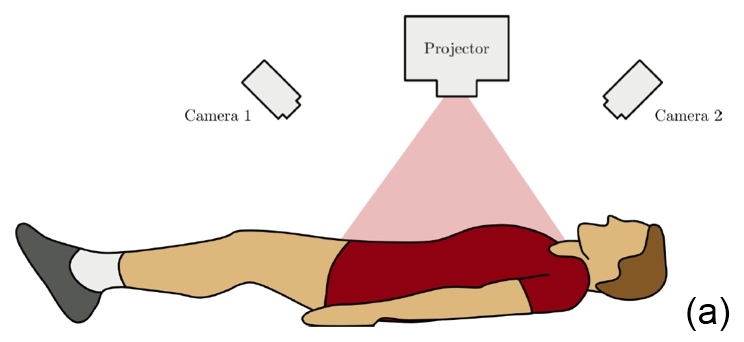
\includegraphics[width=2.2in]{imgs/slp}
  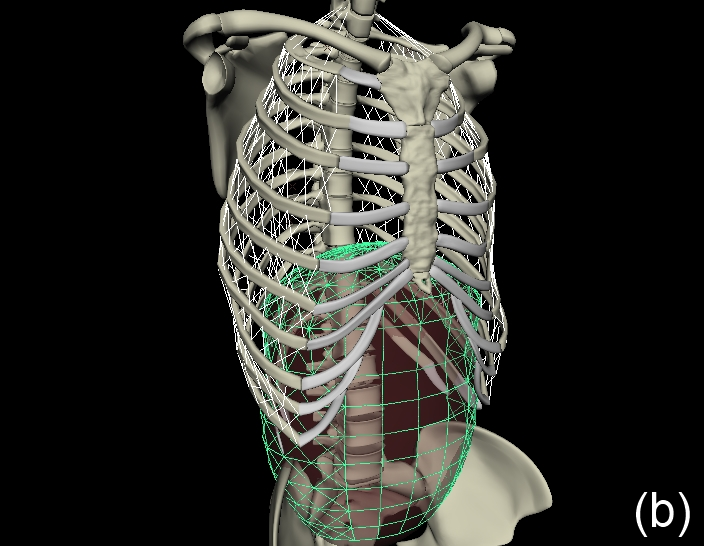
\includegraphics[height=1in]{imgs/skeleton}
  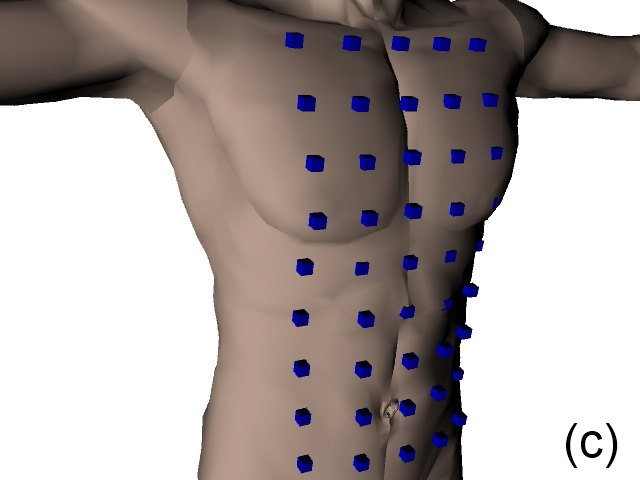
\includegraphics[height=1in]{imgs/skin_grid}
  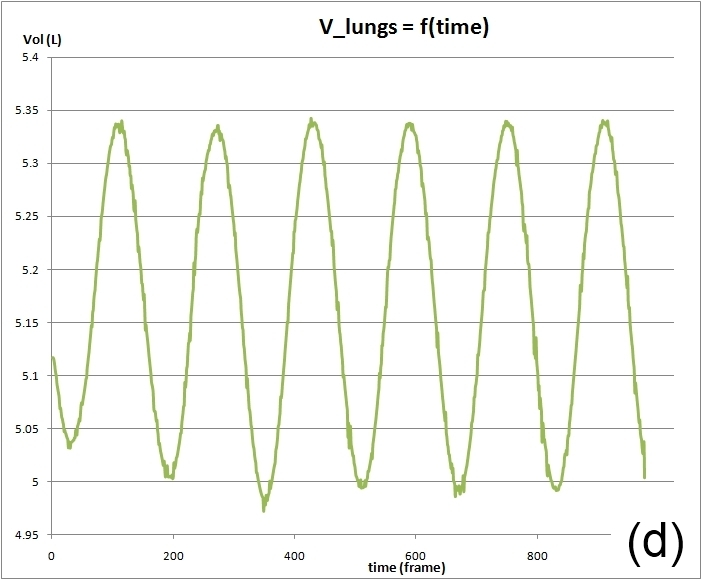
\includegraphics[height=1in]{imgs/v_lungs}
  \caption{(a) SLP: using two cameras, the space coordinates of the corners of a projected grid on a patient's chest are reconstructed (b) 3D model of the human torso: the rib cage muscles (white) and the abdominal muscles (green) (c) the model is fitted to the patient and is driven by the SLP dataset via an optimisation algorithm (d) the simulation provides realistic absolute volume of the lungs.}
}

%% The ``\maketitle'' command must be the first command after the
%% ``\begin{document}'' command. It prepares and prints the title block.

\maketitle


\section{Abstract}
This work describes further research on the Structured Light Plethysmography (SLP) \cite{2010slp} project which is a non-invasive method for pulmonary function testing using visible light. This technique uses two cameras and a known grid which is projected onto the chest of a patient. Using stereo vision algorithms, the 3D coordinates of each grid point projected on the chest wall are recovered over time. As the device captures only the front of the chest wall, we cannot infer the absolute volumes of the lungs but only volume changes of the thoracic cage. However, when it comes to examining respiratory function in a patient, absolute volumes represent a crucial piece of information. In order to address this problem we use optimisation techniques to fit SLP data to a highly detailed 3D model of the human torso (composed of rigid parts and muscles) that we have created. Our simulation provides us with both the optimal muscle inputs to simulate breathing - to date, these muscle activations have remained mysterious and been simplified to sine functions in the literature - and the absolute volumes of the lungs for a given SLP dataset.

As we wish to investigate pulmonary function, the model must be anatomically and physiologically accurate enough to be medically approved. Previous attempts have concentrated more on the visual side of the simulations than on the medical applications, which often resulted in overly simplified models. \cite{lee2009comprehensive} describes a model of the whole upper body but with few respiratory muscles of the rib cage and with no diaphragm, which is an essential muscle in breathing. \cite{zordan2004breathe} uses a skeleton model which anatomically-wise lacks realism and simplifies the articular bones in the spine and the rib cage by grouping and treating them as a single rigid body. Furthermore, the different muscles are grouped and receive the same input (a step function for the diaphragm and sine functions for all the others) in order to produce visually pleasing results.
In comparison, our model has high anatomical accuracy in the dimensions of the rigid parts and in the locations of the joints linking them and the muscles involved in breathing (the rigid parts, the joints and the muscle locations were designed using current anatomy books). In addition, it has high-level controls, is fully tunable (each muscle can be activated independently) and can be fitted to different patient anatomies.

%\section{Our Approach}
Breathing entails expanding (inspiration) and contracting (expiration) the chest wall. From a physiological point of view, this is done through two different moving parts of the body: the rib cage and the abdominal cavity. The rib cage is driven by three types of muscles: the scalene muscles and the external intercostals which expand the rib cage by lifting up the ribs and the internal intercostals which move the rib cage down. The abdominal cavity is put into motion by the diaphragm, which contributes in expanding the lung volume by pushing down the organs inside the abdominal cavity resulting in the ventral abdominal wall moving outwards, and the abdominal muscles, which push the ventral abdominal wall inwards. To model the abdominal breathing, when the diaphragm contracts, the vertices located at the ventral part of the abdominal wall move according to the volume decrease inside the abdominal cavity. In total, we use 510 muscle elements for the rib cage and 270 for the abdominal cavity. Each muscle element is modelled as a spring and a damper in parallel, parameters of which are tuned individually depending on the type of muscle with their activations depending on their lengths. We note that \cite{zordan2004breathe} and \cite{lee2009comprehensive} use the Hill type muscle model. The additional complexity in \cite{lee2009comprehensive}, which uses a FEM of the actual muscle surface, is not appropriate for our respiratory muscles which are just thin layers and do not affect the skin deformation.

We begin by shaping our skeleton model and creating an adapted skin mesh according to anatomical characteristics of the patient. Next, we acquired data of the patient breathing with the SLP technique which gives coordinates of grid points located on the chest of the patient (corrected for projection effects). An optimisation then derives the different muscle activations of our simulation to fit the SLP dataset. Currently, we use the Nelder-Mead Downhill Simplex Method to optimise over several muscle parameters and we use as cost function the distance error over a whole dataset between the grid points of the SLP and their closest vertices on the skin model. Thus, we get the volume of the lungs of our simulation over time and the different activation muscle parameters that drive the breathing. We present results which show the visual realism of the resultant breathing. The validation of our method is done by comparing the simulated lung volumes with spirograms.

\small 
\bibliographystyle{acmsiggraph}
\bibliography{template}
\end{document}
